\chapter{Problem Statement}
\label{chap:planteamientoproblema}

\section{Problem}
The 11th circular letter of the Financial Superintendence of Colombia stipulates that all entities governed by it, should set a money laundering and terrorist financing risk management system (quote). Two methodologies are proposed to try to comply with the standard.
The first comes from building clusters by using the K-Means method, and the second by building decision trees, methodology used in companies (citing training). It is intended to show whether through clusters can achieve an acceptable and applicable classification in the financial field.\par
These methodologies will be applied on the same database and the obtained results will be compared, on the assumption that valid results are obtained from decision trees.
\section{Implementation}
We will now explain the way how decision tree implementation and K-means were developed using the program SPSS.
\subsection{Decision trees}
We will use the SPSS statistical program to elaborate the customer segmentation through classification, decision trees.\par
The decision tree procedure makes a classification model based on trees and classifies cases into groups or predicts values of a dependent variable (standard) based on independent variable values (predictors).\par
The first thing to do is clean the information which is required to elaborate the model. We have a database that provides information such as Income, Assets and six months financial movements. As in most of the cases we find that there are some missing data, in this opportunity some those cases that did not have the necessary information that could affect segmentation were excluded (Asobancaria training).\par
Following the Financial Superintendence suggestions, we will take into account for customer segmentation the following variables:
\begin{itemize}
\item[1.] Incomes
\item[2.] Assets
\item[3.] Credits volume
\end{itemize}
From the variables, asset, income and credit volume we calculate percentiles to round numbers to the nearest unit and be able to establish better groups.
Then we get the following classification for the volume of credits:
\begin{itemize}
\item[*] Lower than 3.000.000
\item[*] Between 3.000.000 and 15.000.000
\item[*] Between 15.000.000 and 30.000.000
\item[*] Between 30.000.000 and 60.000.000
\item[*] Between 60.000.000 and 120.000.000
\item[*] Between 120.000.000 and 210.000.000
\item[*] More than 210.000.000
\end{itemize}
for the variable incomes:
\begin{itemize}
\item[*] Lower than 5.000.000
\item[*] Between 5.000.000 and 10.000.000
\item[*] Between 10.000.000 and 20.000.000
\item[*] Between 20.000.000 and 50.000.000
\item[*] More than 50.000.000
\end{itemize}
for the variable assets:
\begin{itemize}
\item[*] Lower than 50.000.000
\item[*] Between 50.000.000 and 150.000.000
\item[*] Between 150.000.000 and 300.000.000
\item[*] Between 300.000.000 and 500.000.000
\item[*] Between 500.000.000 and 1.000.000.000
\item[*] More than 1.000.000.000
\end{itemize}
Next step consists on running the program.
SPSS asks for a dependent variable that in this case is \emph{Credits volume} (deposits made by every customer) and the independent variables that will be incomes and assets.

SPSS offers the following growing methods for the trees:
\begin{itemize}
\item[1.] CHAID
\item[2.] Exhaustive CHAID
\item[3.] CRT
\item[4.] QUEST
\end{itemize}
We will select CRT due to it divides the data into the most possible homogeneous segments in relation to the dependent variable.
Next graphic will show us the first division of the decision tree made taking into account incomes variable:
\begin{figure}[htbp]
  \centering
  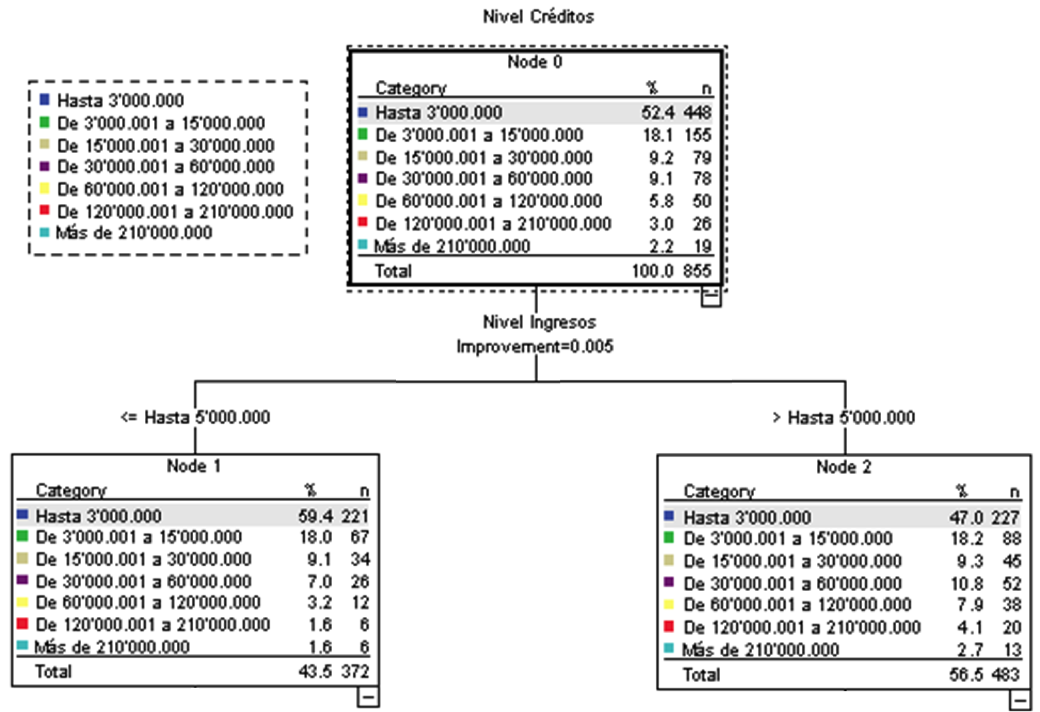
\includegraphics[width=0.95\textwidth]{Imagen1}
  \caption{caption}
  \label{fig:label}
\end{figure}

We analyze the tree’s results and go about the subsequent pruning that corresponds to the CRT algorithm

\begin{figure}[htbp]
  \centering
  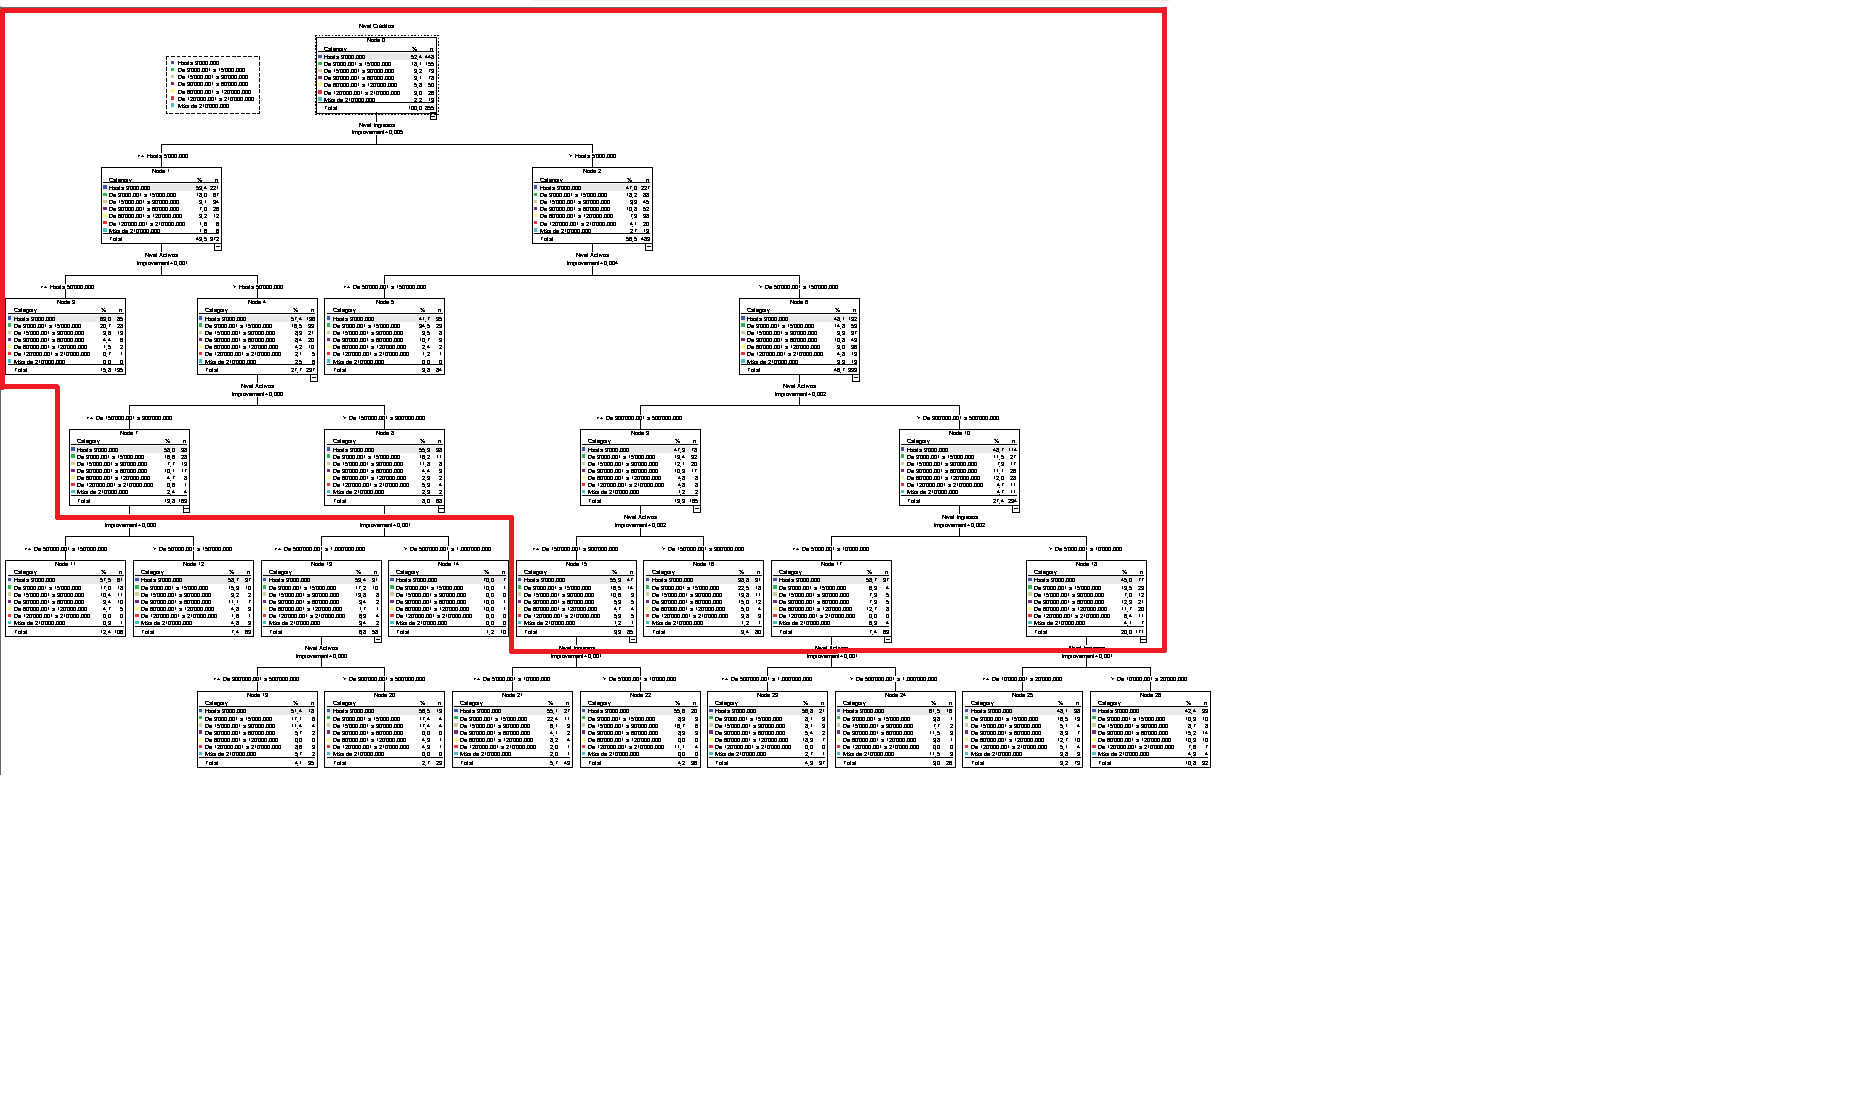
\includegraphics[width=0.95\textwidth]{arbolpodado}
  \caption{caption}
  \label{fig:label}
\end{figure}

\subsubsection{Alerts determination}
For determining the alerts of the obtained segments by mean of the decision trees, we will use the percentages showed by every node of the tree with customer movement’s information:

\begin{figure}[htbp]
  \centering
  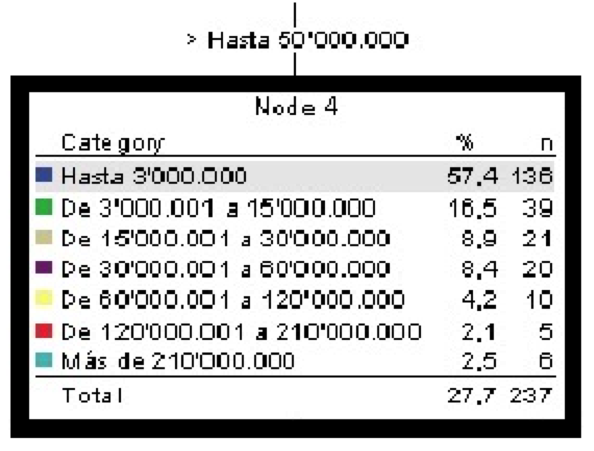
\includegraphics[width=0.95\textwidth]{Segmentoejemplo}
  \caption{caption}
  % \label{fig:label}
\end{figure}

The node shows us how many customers made some kind of movements and indicates the related percentage inside the segment, as well.
In such a way we can say that if a lower percentage of customers make bigger movements than the rest of them, it is a warning sign because it is outside of the movement’s expected range.

 \subsection{K-Means Algorithm}
We will use the SPSS statistical program to elaborate the customer’s classification through K - means.\par
This procedure attempts to identify relatively homogeneous groups of cases based on selected characteristics, using an algorithm that can handle large numbers of cases.  However, the algorithm requires you to specify the number of clusters.  We can specify initial cluster centers if we know this information. In our case, we are going to determine cluster centers iteratively.\par
To use K - means, we have to keep in mind that the variables should be quantitative at the interval or ratio level.  Also, we assume that the distances are computed using simple Euclidean distance.\par
Similarly to what was done with decision trees, we clean the information which is required to elaborate the model. We have a database that provides information such as Income, Assets and six months financial movements. As in most of the cases we find that there is some missing data, in this opportunity some those cases that did not have the necessary information that could affect segmentation were excluded (Asobancaria training).
Following the Financial Superintendence suggestions, we will take into account for customer segmentation the following variables:
\begin{itemize}
\item[1.] Incomes
\item[2.] Assets
\item[3.] Credits volume
\end{itemize}
Similarly to what was done with decision trees, we clean the information which is required to elaborate the model. We have a database that provides information such as Income, Assets and six months financial movements. As in most of the cases we find that there are some missing data, in this opportunity some those cases that did not have the necessary information that could affect segmentation were excluded (Asobancaria training).
for the variable incomes:
\begin{itemize}
\item[*] Lower than 5.000.000
\item[*] Between 5.000.000 and 10.000.000
\item[*] Between 10.000.000 and 20.000.000
\item[*] Between 20.000.000 and 50.000.000
\item[*] More than 50.000.000
\end{itemize}
for the variable assets:
\begin{itemize}
\item[*] Lower than 50.000.000
\item[*] Between 50.000.000 and 150.000.000
\item[*] Between 150.000.000 and 300.000.000
\item[*] Between 300.000.000 and 500.000.000
\item[*] Between 500.000.000 and 1.000.000.000
\item[*] More than 1.000.000.000
\end{itemize}
The variable Credits volume will be use to determine the alerts.
\subsubsection{Alerts determination}
For determining the alerts of the obtained segments by mean of the K - means, we will use the standard deviation of the variable credits volume, will be doing this for each segment.
\clearemptydoublepage
